\documentclass[a4paper]{article}
\usepackage{cmap}
\usepackage{mathtext}
\usepackage{amssymb}
\usepackage{amsmath}
\usepackage[russian]{babel}
\usepackage{indentfirst}
\usepackage[pdftex]{graphicx}
\usepackage{multirow}
\usepackage{mathrsfs}
\usepackage{biblatex}
\usepackage{siunitx}
\usepackage[left=2cm,right=2cm,top=2cm,bottom=2cm]{geometry}
\usepackage{fancyhdr}
\usepackage{float}
\bibliography{bib}
\pagestyle{fancy}
\newcommand{\rref}[1]{(\ref{#1})}
\newenvironment{comment}{}{}
\newcommand{\picref}[1]{рис. \ref{#1}}
\newcommand{\mbf}{\mathbf}
\newcommand{\Equip}[3]{

	{\bf #1:} $\Delta = \pm #2$ \si{#3}}
\newcommand{\equip}[1]{

	{\bf #1}}
\newcommand{\labname}{Фазовая дифракционная решётка} 	% название пиши здесь
\newcommand{\labnum}{4.4.2}		% номер вводи здесь
\fancyfoot{}
\fancyhead[RE, RO]{\thepage}
\fancyhead[LE, LO]{Лабораторная работа \labnum \space \labname}
\title{Лабораторная работа \labnum \space \labname} % Название работы здесь
\author{Балдин Виктор}
\begin{document}
\maketitle
\thispagestyle{empty}
\section{Аннотация}
В данной работе проводится  знакомство с работой и настройкой гониометра Г5, определение спектральных характеристик фазовой решётки (эшелетта) и исследование спектра ртутной лампы.

\section{Теоретические сведения}

\begin{figure}[tbp]
	\centering
	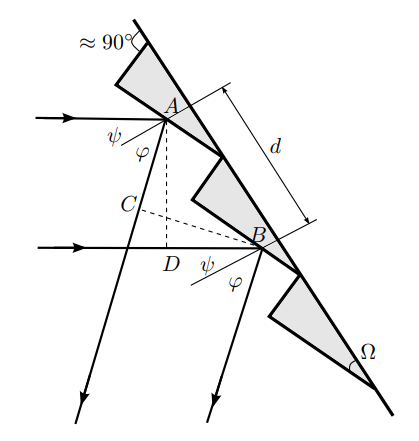
\includegraphics[width=0.8\linewidth]{Screenshot_2}
	\caption{Профиль фазовой дифракционной решётки; дифракция световой волны}
	\label{fig:решёткаВпрофиль}
\end{figure}

В современных спектральных приборах широко используются отражательные решётки с треугольным профилем штриха (рис. \ref{fig:решёткаВпрофиль}), они способны концентрировать до $ 70–80\% $ падающего излучения в рабочий порядок спектра. Отражательная решётка, в которой угол $ \Omega $ между рабочей гранью и плоскостью решётки не превышает $ 20^\circ $, называется эшелеттом. Для эшелетта, варьируя угол скоса и шаг решётки, получают рабочий порядок $ m_р \le 10 $.

Найдём разность хода между лучами на рис. \ref{fig:решёткаВпрофиль}. Условие возникновения спектра порядка $ m $:
\begin{equation}\label{eq:spectreM}
	A C - B D = d (\sin \varphi m- \sin \psi) = m \lambda,
\end{equation}
где $ \psi $ -- угол падения от нормали к решётке, $ \varphi $ -- угол дифракции.
Для нулевого порядка $ \varphi_0 = \psi $. В отличие от амплитудной решётки, нулевой порядок не будет самым ярким. Угол $ \varphi_б $ -- угол блеска, соответствующий максимуму интенсивности света, равен углу зеркального отражения падающей волны от одной ступеньки:
\begin{equation*}\label{key}
	\varphi_б = \psi+ 2 \Omega.
\end{equation*}
Для эшелетта рабочим порядком спектра $  m_р$ будет то целое число, которое соответствует минимальной ошибке решения уравнения $d \sin \varphi_m - \sin \psi = 0 $.

Cчитая, что эшелетт работает в автоколлимационном режиме, то есть свет падает перпендикулярно рабочей грани решётки ($ \psi = -\Omega $) и отражается в обратном направлении ($ \varphi = \Omega $), тогда
\begin{equation}\label{om}
	2 d \sin \Omega = m_р \lambda_р.
\end{equation}
В автоколлимационном режиме дифракция на одной ступеньке-зеркальце описывается так же, как и дифракция на отдельной щели амплитудной решётки с максимумом вблизи $ \varphi \approx 0 $. В отличие от амплитудной решётки, нумерацию порядков для амплитудной решётки, следует сместить на величину $ m_р $.

\subsection{Расчётные формулы}

Основные формулы, используемые в работе: \eqref{eq:spectreM}, \eqref{om}. %Вторая часть формулы (1) используется для определния периода $ d $ в МНК на графике рис. 2.

\section{Оборудование и инструментальные погрешности}

\Equip{Гониометр}{1}{''}
\equip{Эшелетт}: $ \lambda_р = \SI{500}{\nano \metre} $ в 1-м порядке.
\equip{Ртутная лампа}

\section{Ход работы}
\subsection{Качественные наблюдения}
Удерживая эшелетт в вытянутой руке, найдите отражённое изображение
нити лампы накаливания, расположенной за вашей спиной.
Вращая эшелетт, наблюдайте спектры различных положительных и отрицательных
порядков. Определите рабочий порядок, в котором спектр
наиболее интенсивен. Отметьте ориентацию направлений: источник
света–эшелетт, эшелетт–направление на рабочий спектр. При прове-
дении опытов это будут направления: коллиматор–эшелетт, эшелетт–
зрительная труба.
Отметьте, в каких порядках спектры начинают перекрываться. Оцените
для этих порядков дисперсионную область и сравните её с (4.21)
для средней длины волны 500 нм и полуширины 200 нм, что соответствует
наблюдению глазом излучения лампы накаливания. Запишите
паспортные данные эшелетта: рабочий порядок mp, рабочую длину волны
$\lambda_p$.

\subsection{Установка эшелетта}
Основание оправы эшелетта и его ступеньки могут быть не перпендикулярны
друг другу, поэтому плоскость столика следует немного
наклонить.
\begin{enumerate}
  \item Настройте зрительную трубу на наблюдение входной щели коллиматора,
  вертикальный размер изображения щели должен быть менее половины
  поля зрения, рекомендуемый начальный отсчёт угла 180◦. Вам
  известны направления: ось коллиматора–эшелетт–рабочий порядок, поверните
  алидаду на 120◦ от начального положения, направление вращения,
  вправо или влево, должно позволить наблюдать рабочий порядок.
  \item Поставьте эшелетт на столик рабочей поверхностью к коллиматору так,
  чтобы эшелетт был параллелен одному из винтов 8 и перпендикулярен
  другому. Вращая только верхнюю часть столика, освободив винт 27
  (винт 26 закреплён, чтобы не сбился начальный отсчёт угла), найдите
  ахроматическое (белое) изображение щели коллиматора, отражённое
  от эшелетта (спектр нулевого порядка). При этом угол падения света
  на плоскость эшелетта $\psi = (180^{\circ} - 120^{\circ})/2 = 30^{\circ}$.
  \item Винтом 8, перпендикулярным плоскости эшелетта, совместите центр
  изображения щели с горизонтальным штрихом отсчётного креста окуляра
  зрительной трубы. Отводя алидаду от коллиматора, найдите изображение
  линии в дальнем порядке и вторым винтом 8, параллельным
  плоскости эшелетта, устраните вертикальное расхождение. Вернитесь
  к ахроматическому изображению и уточните положение винтов 8 по
  приведённой процедуре. Допустимое вертикальное смещение линий --
  менее трети радиуса поля зрения.
\end{enumerate}

\subsection{Исследование спектра ртутной лампы}
\begin{enumerate}
  \item Подберите ширину входной щели коллиматора, при которой ширина
  линий жёлтого дублета чуть больше промежутка между линиями двойного
  штриха зрительной трубы. Установите высоту щели, удобную для
  измерений (при короткой щели плохо виден двойной штрих, при слишком
  высокой -- мешает кривизна изображения).
  \item Для угла падения $\psi = 30^{\circ}$ измерьте угловые координаты спектральных
  линий ртути в рабочем порядке. Примерное расположение и относительная
  яркость основных линий приведены в Приложении (рис. П4.4,
  табл. 1).
  \item Для оценки разрешающей способности спектрального прибора измерь-
  те угловую ширину одной из линий жёлтого дублета (по нулям ин-
  тенсивности). Ширина щели коллиматора должна быть минимальной,
  позволяющей провести измерения.
  \item Для установленного угла падения $\psi = 30^{\circ}$ измерьте угловые координа-
  ты жёлтого дублета во всех наблюдаемых порядках, положительных и
  отрицательных. Эти данные позволят оценить дисперсию в различных
  порядках спектра для фиксированного угла падения.
  \item Измерьте угловые координаты линий жёлтого дублета в рабочем по-
  рядке для углов падения 45\textdegree и 60\textdegree. Для больших углов падения есть
  возможность найти изображение автоколлимационного креста, отражённого
  от эшелетта. В этом положении ось зрительной трубы перпендикулярна
  плоскости эшелетта, и можно ввести ещё одно удобное
  начало отсчёта углов. Например, угол падения света равен углу наблюдения
  ахроматической полосы, отсчитанному от нового начала.
  Обратите внимание на появление спектров больших отрицательных
  порядков при увеличении угла падения света.
  \item Эшелетт, ширина штриха которого сравнима с длиной волны, поляризует
  отражённый свет. Проведите следующий эксперимент. Используя
  отдельный эшелетт с плотностью штрихов 1200 штрихов/мм (полное
  число штрихов 180 000, ширина отдельного штриха меньше 1 мкм), а
  в качестве источника излучения -- свет настольной лампы (излучение
  имеет случайную поляризацию), определите с помощью поляроида преимущественное
  направление колебания электрического вектора в пер-
  вом порядке спектра. Как связаны между собой это направление и ори-
  ентация штрихов? Объясните этот эффект.
\end{enumerate}

\section{Результаты измерений и обработка данных}
\emph{Все измерения и расчёты в СИ.}

Произведём юстировку гониометра и установим начало отсчёта, руководствуясь техническим описанием.11321

Держа эшлет в вытянутой руке, найдём отражение лампы накаливанияж вращая эшелет вокруг оси, рассмотрим спектры положительных и отрицательных порядков; определим рабочий порядок; оценим дисперсионную область и сравним её с шириной спектра лампы:

\noindent
Средние значения:
\[
	\lambda = 600\ нм; \quad \Delta \phi = 200\ нм;
\]
\[
	G = \frac{\lambda}{m} = 200\ нм; \quad \text{Рабочий порядок}\ m_p = -1.
\]
Проделаем дополнительную настройку столика с эшелетом; установим $\psi = 30^o$; подберём ширину входной щели так, чтобы хорошо разрешались линии жёлтого дублета (ширина изображения щели чуть больше промежутка между линиями двойного штриха); установим высоту щели, удобную для измерений.

Для угла $\psi = 45^o$ измерим угловые координаты спектральных линий ртути в рабочем порядке. Отметим гловую координату каждой из описанных линий:
\begin{table}[H]
\centering
\begin{tabular}{|c|c|c|}  \hline
Ахроматический & $93^o 10' 30''$ & {} \\\hline
Фиолетовый & $75^o 36' 45''$ & $4047 \dot A$ \\\hline
Синий & $74^o 23' 45''$ & $4358 \dot A$ \\\hline
Голубой & $72^o15'35''$ & $4916 \dot A$ \\\hline
	Зелёный & $70^o12'35''$ & $5461 \dot A$ \\\hline
Желтый 2 & $69^o 3' 25''$ & $5770 \dot A$ \\\hline
Жёлтый 1 & $68^o 58'35''$ & $5791 \dot A$ \\\hline
\end{tabular}
\end{table}
Для оценки разрешающей способности измерим гирину одной из линий жёлтого дублета и рассчитаем аппаратную полуширину линии $\Delta \lambda$:
\[
\text{Ширина линии:}\ 68^o2'10'' - 68^o2'0'' = 10''
\]
\[
\Delta \lambda = \frac{1}{3} \dot A; \quad R = \frac{\lambda}{\Delta \lambda} =\frac{5770}{20} \cdot 60 =  17810
\]
Для угла $\psi = 30^o$ измерим координаты каждой из жёлтых линий во всех наблюдаемых порядках:
\begin{table}[H]
\begin{center}
\begin{tabular}{|c|c|c|} \hline
& $Ж_1$ & $89^o3'55''$ \\
\cline{2-3}
$I_{пол}$
& $Ж_2$ & $88^055'45''$ \\\hline
& $Ж_1$ & $39^o50'55''$ \\
\cline{2-3}
$I_{отр}$
& $Ж_2$ & $39^o55'25''$ \\\hline
\end{tabular}
\end{center}
\end{table}
Повторим измерения для $\psi = 45^0, 60^o$:

\begin{table}[H]
\begin{center}
\begin{tabular}{|c|c|c|} \hline
& $Ж_1$ & $68^058'35''$\\
\cline{2-3}
$I_{отр}$
& $Ж_2$ & $69^o3'35''$ \\\hline
& $Ж_1$ & $48^o32'15''$ \\
\cline{2-3}
$II_{отр}$
& $Ж_2$ & $48^o40'50''$ \\\hline
\end{tabular}
\caption{$\psi = 45^o$}
\end{center}
\end{table}

\begin{table}[H]
\begin{center}
\begin{tabular}{|c|c|c|} \hline
& $Ж_1$ & $92^o15'5''$\\
\cline{2-3}
$I_{отр}$
& $Ж_2$ & $92^o20'15''$ \\\hline
& $Ж_1$ & $70^o51'45''$ \\
\cline{2-3}
$II_{отр}$
& $Ж_2$ & $71^o0'35''$ \\\hline
& $Ж_1$ & $50^o51'5''$\\
\cline{2-3}
$III_{отр}$
& $Ж_2$ & $51^o4'45''$ \\\hline
\end{tabular}
\caption{$\psi = 60^o$}
\end{center}
\end{table}
\textbf{Зависимость разрешающей силы от ширины пучка:}

Натроим зрительную трубу на желтый дублет в рабочем порядке; определим начало отсчёта "--- момент открытия щели. Крест появляется при $59^o57'20''$; ширина щели "--- 3 деления.

Откроем щель пошире; уменьшая ширину щели, добьемся предельного разрешения желтого дублета, оценим число штрихов:
\[
	 n \approx 1600\ штр/мм; \quad \Delta \lambda = 2 \dot A.
\]
Построим график зависимости $\sin \varphi_m = f(\lambda)$ и по углу наклона определим период эшелета:
\begin{figure}[h]
	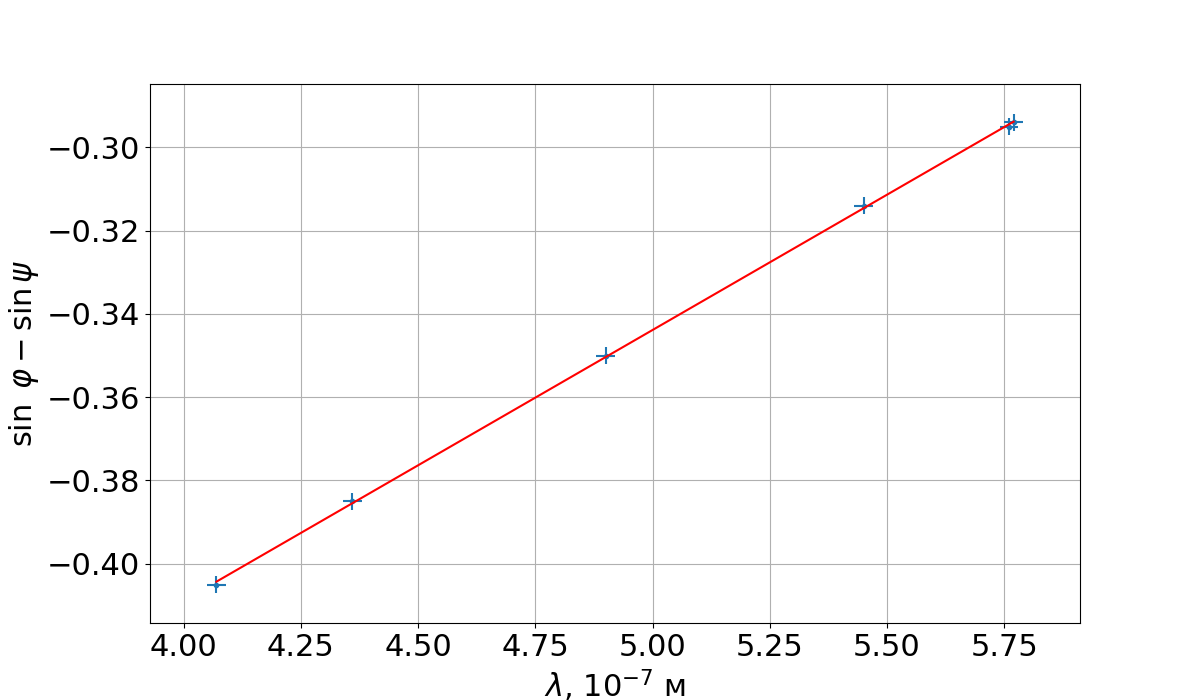
\includegraphics[width = 1.0\linewidth]{g1.png}
	\caption*{Зависимость $\sin \varphi_m$ от $\lambda$}
\end{figure}
Угол наклона графика $k = (6.5 \pm 0.1)\cdot 10^6$

Число штрихов $n \approx 650 \pm 10\ штр/мм$

Период эшелета: $d = \frac{1}{0.65} = 1.53 \pm 0.04$ мм.

Угловая дисперсия в рабочем порядке для жёлтого дублета в угловых секундах на $\dot A$:
\[
D = 14.3\ \frac{угл \cdot сек}{\dot A}
\]
Экспериментальная разрешающая способность:
\[
R = \frac{\lambda}{\Delta \lambda} = 2890
\]

\subsection{Оценка погрешностей}

Как и обычно, оценка инструментальных погрешностей проводится по общей формуле (с частными производными); в экспериментах с несколькими измерениями случайные погрешности существенно превалируют над инструментальными.

\section{Вывод}

Судя по расхождению экспериментальных данных с теоретическими, при снятии показаний гониометра, несмотря на его точность, были допущены ошибки, в частности, при измерении расстояния между жёлтыми спектральными линиями. Отчасти это связано с неудобством снятия показаний.

Тем не менее, удалось с неплохой точностью найти характеристики дифракционной решётки и исследовать спектр ртутной лампы.

\newpage
\begin{thebibliography}{9}
	\bibitem{Siv} Сивухин Д. В. \emph{Общий курс физики. Том 4 Оптика}, 2004
	\bibitem{kir} Кириченко Н. А. \emph{Принципы оптики}, 2014
	\bibitem{max} \emph{Лабораторный практикум по общей физике. В 3 томах. Том 2. Оптика: учебное пособие} под ред. А. В. Максимычева
\end{thebibliography}
\end{document}